
\documentclass[11pt]{article}
\usepackage[margin=1in]{geometry}
\usepackage{amsmath,amssymb}
\usepackage{graphicx}
\usepackage{booktabs}
\usepackage{array}
\usepackage{float}
\usepackage{hyperref}
\title{A Maturity-Governed Rotational Support Hypothesis for Disk Galaxies: Preliminary Tests and Falsifiable Predictions}

\author{Jake Enholm}
\date{}
\begin{document}
\maketitle

\begin{abstract}
\textbf{Established input.} SPARC supplies baryonic masses, observed flat rotation velocities, gas fractions, surface-density proxies, and H~I extent measures for a quality-controlled disk-galaxy sample; some galaxies occupy different locations relative to the mature BTFR scale. Decisive same-object resolved H~I morphology and kinematic measurements are not yet available for a sufficiently complete homogeneous sample, so the present work is a preliminary scalar diagnostic rather than a confirmation of the mechanism. \textbf{Preliminary result.} We ask whether a maturity-dependent BDVR governor hypothesis can order the normalized support residual $A_{\rm inferred}$ using only $f_*$, $\Sigma_b$, $f_{\rm gas}$, and $R_{\rm H\,I}/R_d$. The selected product gate gives modest ordering with substantial unexplained scatter: MSE=0.183 and Spearman $\rho=0.146$. The result is further limited because the clipped target has 12 galaxies at 0, 6 at 1, and only 69 galaxies in the open interval. \textbf{Unproven prediction.} Resolved H~I morphology, velocity-field symmetry, velocity dispersion, and settling measurements should distinguish low-activation from mature-response systems. External surveys are therefore used as proxy context and candidate-selection channels, not as tests or validation of the governor.
\end{abstract}

\section{Introduction}

The empirical regularity of disk-galaxy rotation remains a central clue in galaxy astrophysics. The baryonic Tully-Fisher relation (BTFR) and the radial acceleration relation (RAR) show that baryons and rotational response are tightly organized, while SPARC makes it possible to inspect how flat velocities relate to gas fraction, surface density, morphology, and H~I extent. The question pursued here is narrower than a full galaxy-dynamics theory: can a maturity-dependent governor hypothesis generate a falsifiable ordering of disk-galaxy rotational support?

We adopt a bound-domain vacuum response (BDVR) formalism in which galaxy-scale rotational support includes an effective response that may activate with baryonic organization. The physical hypothesis is that a dynamically organized bound baryonic disk may receive additional effective rotational support, and that the response may depend on structural maturity. The empirical diagnostic in this paper is deliberately weaker: bounded logistic factors built from $f_*$, $\Sigma_b$, $f_{\rm gas}$, and $R_{\rm H\,I}/R_d$ define a phenomenological test surface.

\begin{center}
\fbox{\begin{minipage}{0.88\textwidth}
\textbf{Operational definition.} Dynamically immature or low-organization state denotes a gas-rich, weakly converted, low-activation state. The shorthand juvenile is used sparingly and does not require youth in cosmic time.
\end{minipage}}
\end{center}

This paper does not claim that the governor hypothesis has been confirmed. The available scalar data permit a preliminary test of whether maturity-related variables can order the inferred rotational response, but they do not provide the resolved same-object H~I and kinematic measurements required to establish the proposed mechanism. The principal result is therefore a falsifiable observational specification: the hypothesis predicts that low inferred activation should coincide with gas-rich, extended, asymmetric, or dynamically unsettled disks, while mature activation should coincide with coherent rotational support. The required measurements are identified here as the next test rather than assumed to exist.

\section{Physical Hypothesis and Claim Boundary}

The physical hypothesis is not a validation claim: a dynamically organized bound baryonic disk may receive additional effective rotational support, and the response may depend on structural maturity. The empirical diagnostic is the bounded product gate below. It is a phenomenological test surface, not derived from an action or fundamental field equation.

\section{SPARC Sample and Measured Quantities}

The SPARC diagnostic sample supplies $v_{\rm obs}$, baryonic mass components, disk scale lengths, gas fractions, surface-brightness proxies, and H~I extent where available. We use $r_{\rm eval}$ as the SPARC flat-velocity/evaluation radius associated with the tabulated outer velocity diagnostic. The baryonic mass convention is $M_{\rm bar}=M_*+1.33M_{\rm H\,I}$; H~I masses are multiplied by 1.33 to account for helium. Stellar masses use the SPARC 3.6 micron stellar mass-to-light ratio $\Upsilon_{3.6}=0.5$, and bulge mass is included when present in the SPARC baryonic mass.

\section{Velocity Normalization and Inferred Activation}

We write the flat-velocity governor equation as
\begin{equation}
  v_{\rm flat}^2 = v_N^2 + A_{\rm inferred} Q_{\rm eff} \sqrt{G M_{\rm bar} a_0},\qquad 0\le A_{\rm inferred}\le 1 .
\end{equation}
Here $v_N$ is the Newtonian baryonic circular speed at $r_{\rm eval}$, $v_{\rm obs}$ is the observed SPARC flat velocity, $v_{\rm full}$ is the full-response BDVR velocity scale, and $a_0=1.2\times10^{-10}\,\mathrm{m\,s^{-2}}$ is the acceleration scale used in the BTFR-like response term. For this scalar diagnostic we set $Q_{\rm eff}=1$ as a normalization convention for all galaxies, so the full-response velocity scale is
\begin{equation}
  v_{\rm full}^2=v_N^2+\sqrt{G M_{\rm bar} a_0} .
\end{equation}
A physical structural-response model would have to specify $Q_{\rm eff}$ independently before Equation (1) could be predictive. In this paper, $Q_{\rm eff}$ is not fitted per galaxy and is not used to tune $A_{\rm inferred}$. The analysis uses three related but distinct quantities:
\begin{enumerate}
\item $\alpha_{\rm BTFR}$ is purely empirical: the observed response relative to the BTFR scale,
\begin{equation}
  \alpha_{\rm BTFR}=\left(\frac{v_{\rm obs}^4}{G M_{\rm bar}a_0}\right)^{1/2} .
\end{equation}
\item $A_{\rm inferred}$ is the observed support requirement, a normalized residual under the assumed BDVR velocity decomposition, renormalized by $v_N^2$ and clipped to $[0,1]$:
\begin{equation}
  A_{\rm inferred} = {\rm clip}_{[0,1]}\left[\frac{v_{\rm obs}^2-v_N^2}{v_{\rm full}^2-v_N^2}\right].
\end{equation}
When $v_{\rm obs}^2<v_N^2$, $A_{\rm inferred}$ is set to 0; when $v_{\rm obs}^2>v_{\rm full}^2$, it is set to 1.
\item $A_{\rm pred}$ is the model prediction based on maturity gates. It asks how much support the governor hypothesis predicts from $f_*$, $\Sigma_b$, $f_{\rm gas}$, and $R_{\rm H\,I}/R_d$, without using the observed rotation endpoint.
\end{enumerate}

\section{Phenomenological Maturity-Gate Model}

The logistic function used by each gate is
\begin{equation}
  \sigma(x;x_c,k)=\frac{1}{1+\exp[-k(x-x_c)]} .
\end{equation}
The product-gate model is
\begin{equation}
  A_{\rm pred}=A_* A_\Sigma A_{\rm gas} A_{\rm H\,I},
\end{equation}
with $A_* = \sigma(f_*; f_{*,c}, k_*)$, $A_\Sigma=\sigma(\log\Sigma_b; \log\Sigma_{b,c}, k_\Sigma)$, $A_{\rm gas}=1-\sigma(f_{\rm gas}; f_{\rm gas,c}, k_{\rm gas})$, and $A_{\rm H\,I}=1-\sigma(R_{\rm H\,I}/R_d; (R_{\rm H\,I}/R_d)_c, k_{\rm H\,I})$. Stellar conversion and surface-density buildup open the gate; high gas fraction and extended H~I suppress it.

\section{Preliminary SPARC Results}


\begin{figure}[t]
\centering
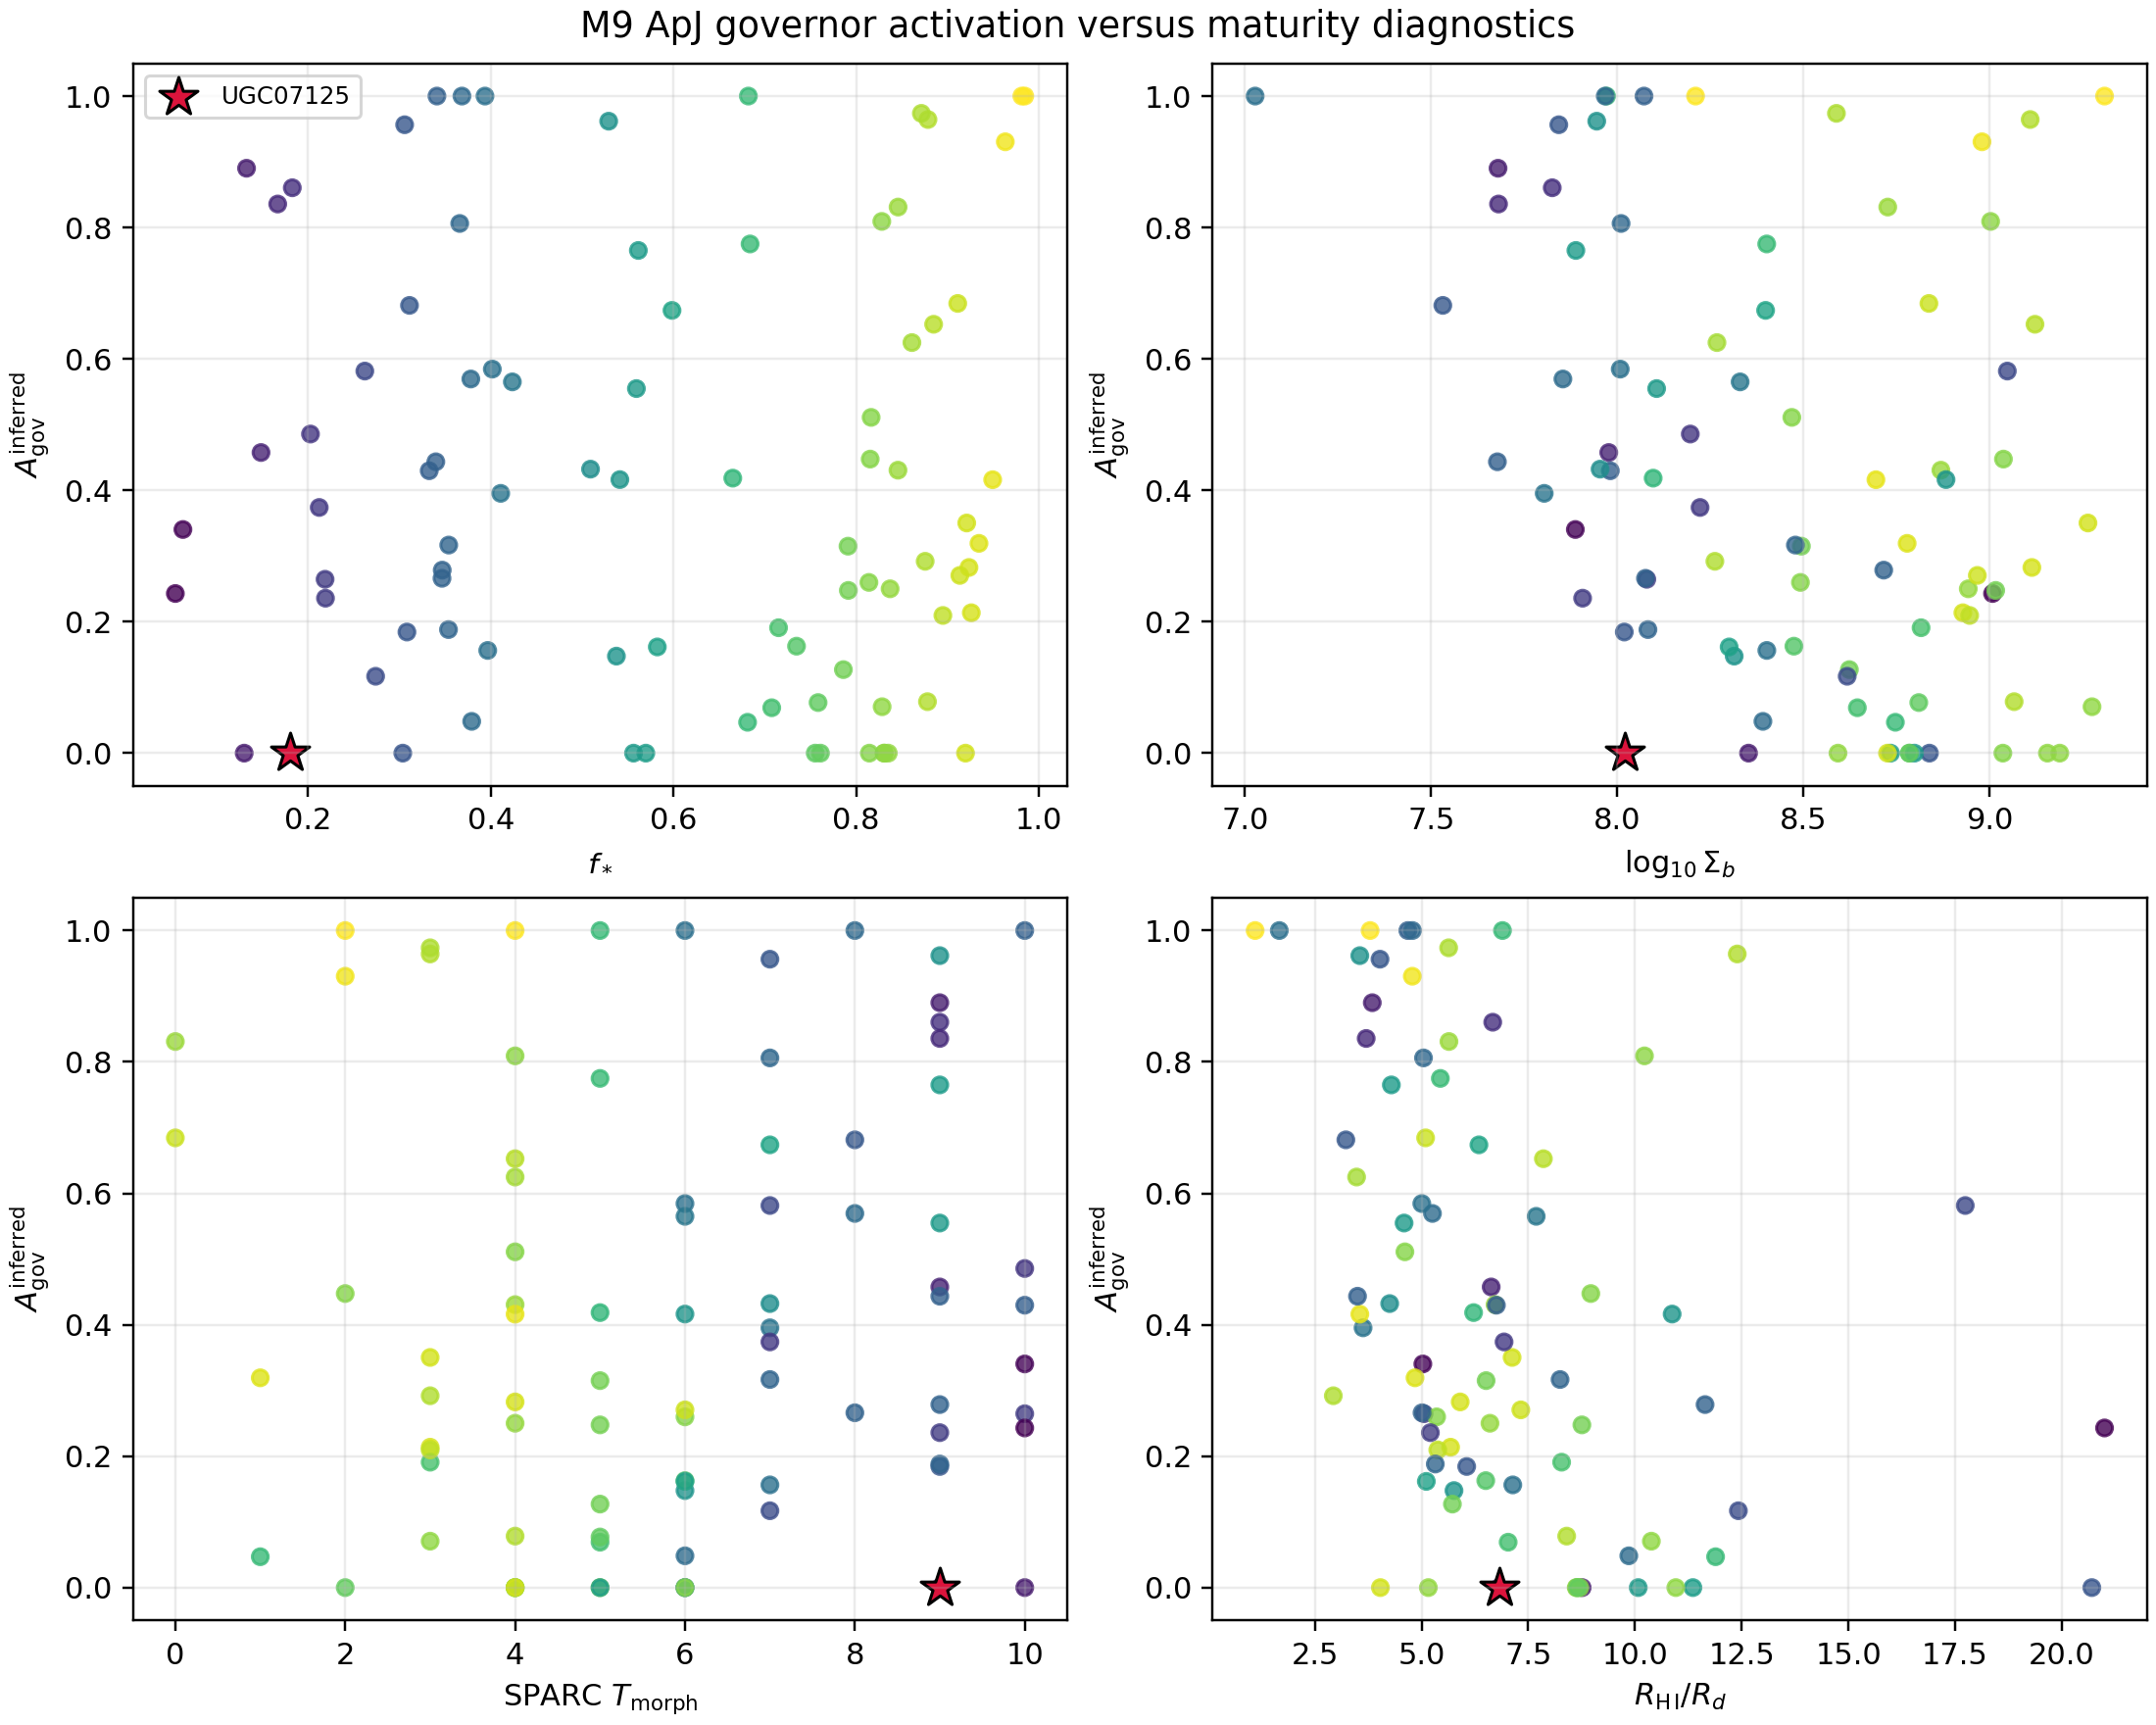
\includegraphics[width=0.92\linewidth]{figures/fig_1_activation_vs_maturity.png}
\caption{Marginal maturity diagnostics for the SPARC diagnostic sample (N=87). \textbf{Clipping warning:} inferred activation has strong boundary concentrations; see Section 7 for the numerical clipping audit. These panels are marginal diagnostics rather than independent tests, and the boundary concentrations should not be over-interpreted. Spearman correlations are rho(fstar)=-0.014, rho(fgas)=0.014, rho(log Sigma b)=-0.364, rho(T)=0.082, and rho(RHI/Rd)=-0.500.}
\label{fig:activation-maturity}
\end{figure}


Across the current SPARC diagnostic sample, maturity-class predicted-activation summaries are: juvenile: N=12, median $A_{\rm pred}$=0.042; mature: N=36, median $A_{\rm pred}$=0.555; transition: N=39, median $A_{\rm pred}$=0.349. The single-variable correlations with $A_{\rm inferred}$ are modest, which is expected if activation is not controlled by one maturity coordinate alone. The useful separation appears only when the gates are combined. In the product model, juvenile systems are strongly suppressed, transition systems sit near the middle of the switch, and mature systems move into the higher-response channel. The diagnostic result is not ``stellar fraction alone controls the response.'' The result is that gas-rich, weakly converted, H~I-extended systems fail the combined maturity gate, while compact and more settled disks are allowed into the mature rotational-support channel.

\begin{table}[H]
\centering
\caption{Excluded asymmetric scalar case retained as a follow-up target.}
\begin{tabular}{lrrrrrr}
\toprule
Galaxy & $f_*$ & $f_{\rm gas}$ & $R_{\rm H\,I}/R_d$ & $\alpha_{\rm BTFR}$ & $A_{\rm inferred}$ & $A_{\rm pred}$ \\
\midrule
UGC07125 & 0.180 & 0.820 & 6.82 & 0.389 & 0.000 & 0.057 \\
\bottomrule
\end{tabular}
\end{table}

UGC07125 is excluded from clean scalar model tests after the published geometry audit. Its scalar coordinates are reported for transparency: $f_*=0.180$, $f_{\rm gas}=0.820$, $R_{\rm H\,I}/R_d=6.82$, $\alpha_{\rm BTFR}=0.389$, $A_{\rm inferred}=0.000$, and $A_{\rm pred}=0.057$. Published observations indicate side-dependent H~I and stellar geometry: the W side is warped, while the E side is not warped; DDO161 is the cleaner juvenile-forming contrast.


\begin{figure}[t]
\centering
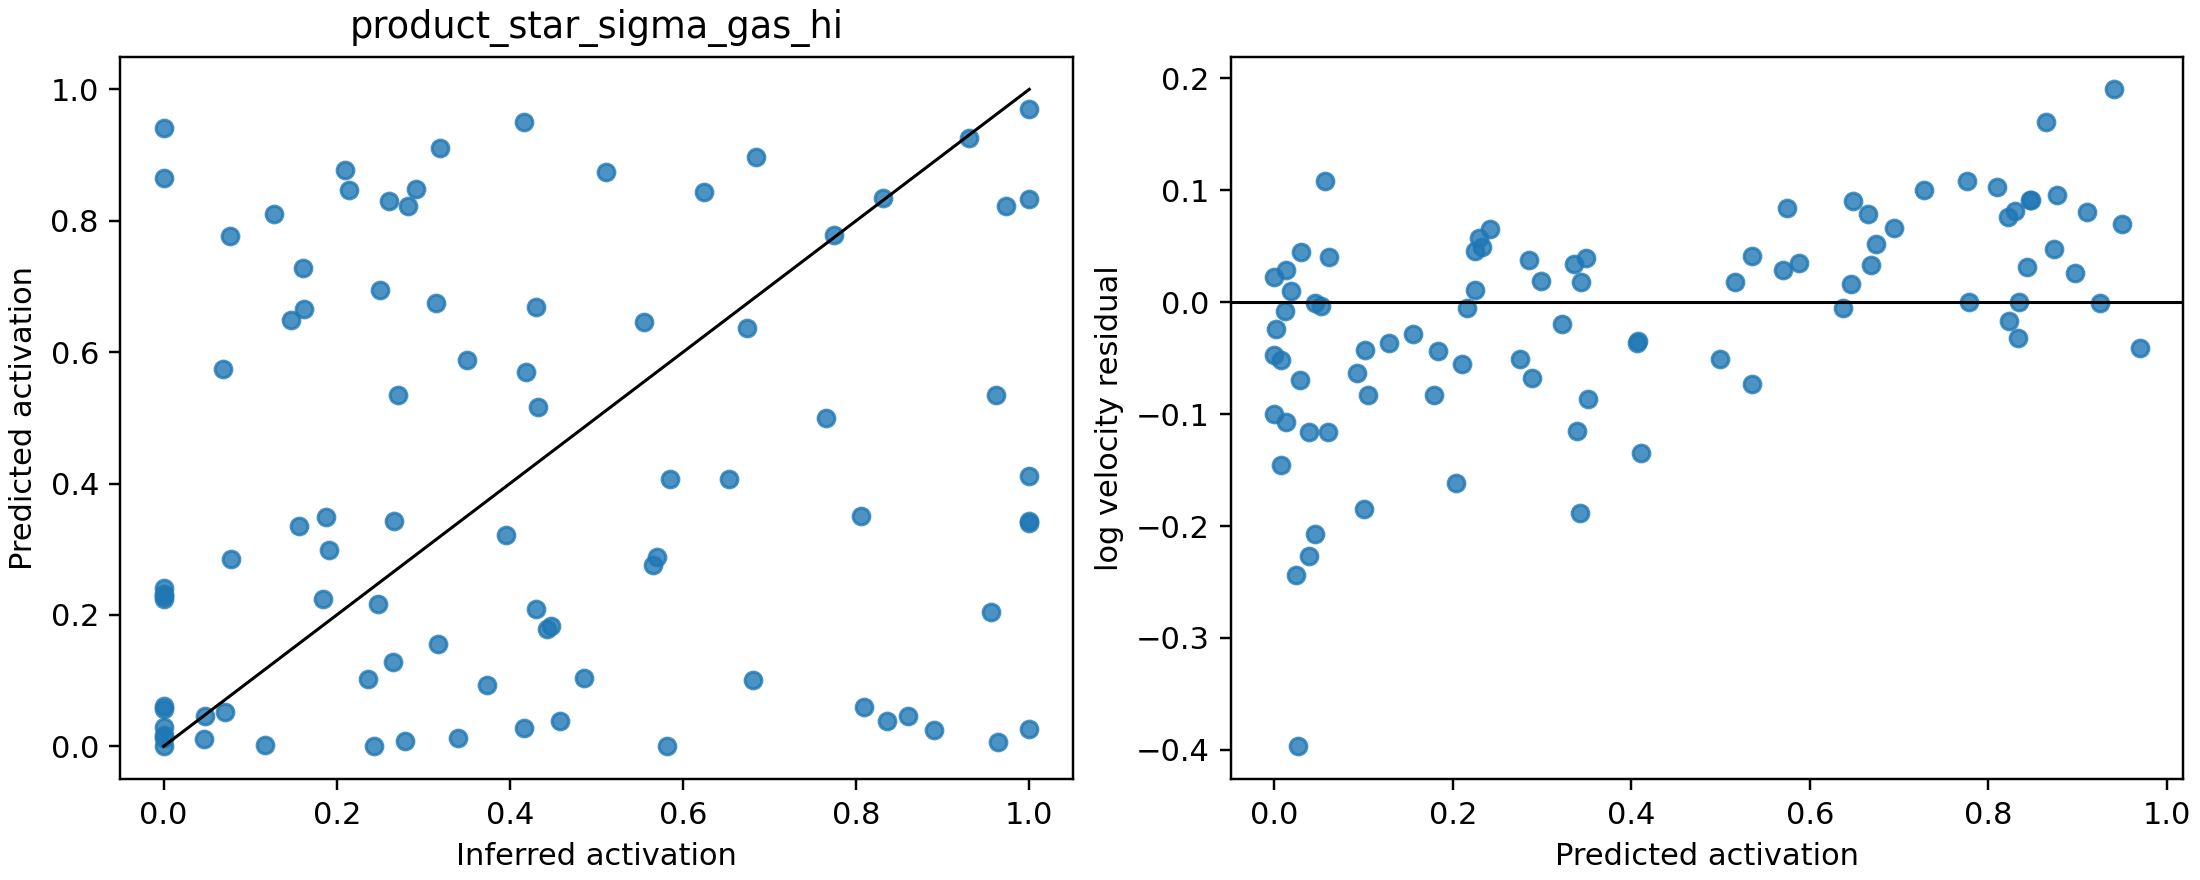
\includegraphics[width=0.92\linewidth]{figures/fig_3_governor_prediction_residuals.png}
\caption{Predicted versus inferred activation. This is the core preliminary diagnostic: predicted activation is computed from maturity gates, while inferred activation is computed from the observed velocity endpoint. The identity line and baseline comparisons should be read against the broad scatter; the current scalar product gate provides only modest predictive ordering and does not constitute confirmation of the governor hypothesis.}
\label{fig:governor-residuals}
\end{figure}



\begin{figure}[t]
\centering
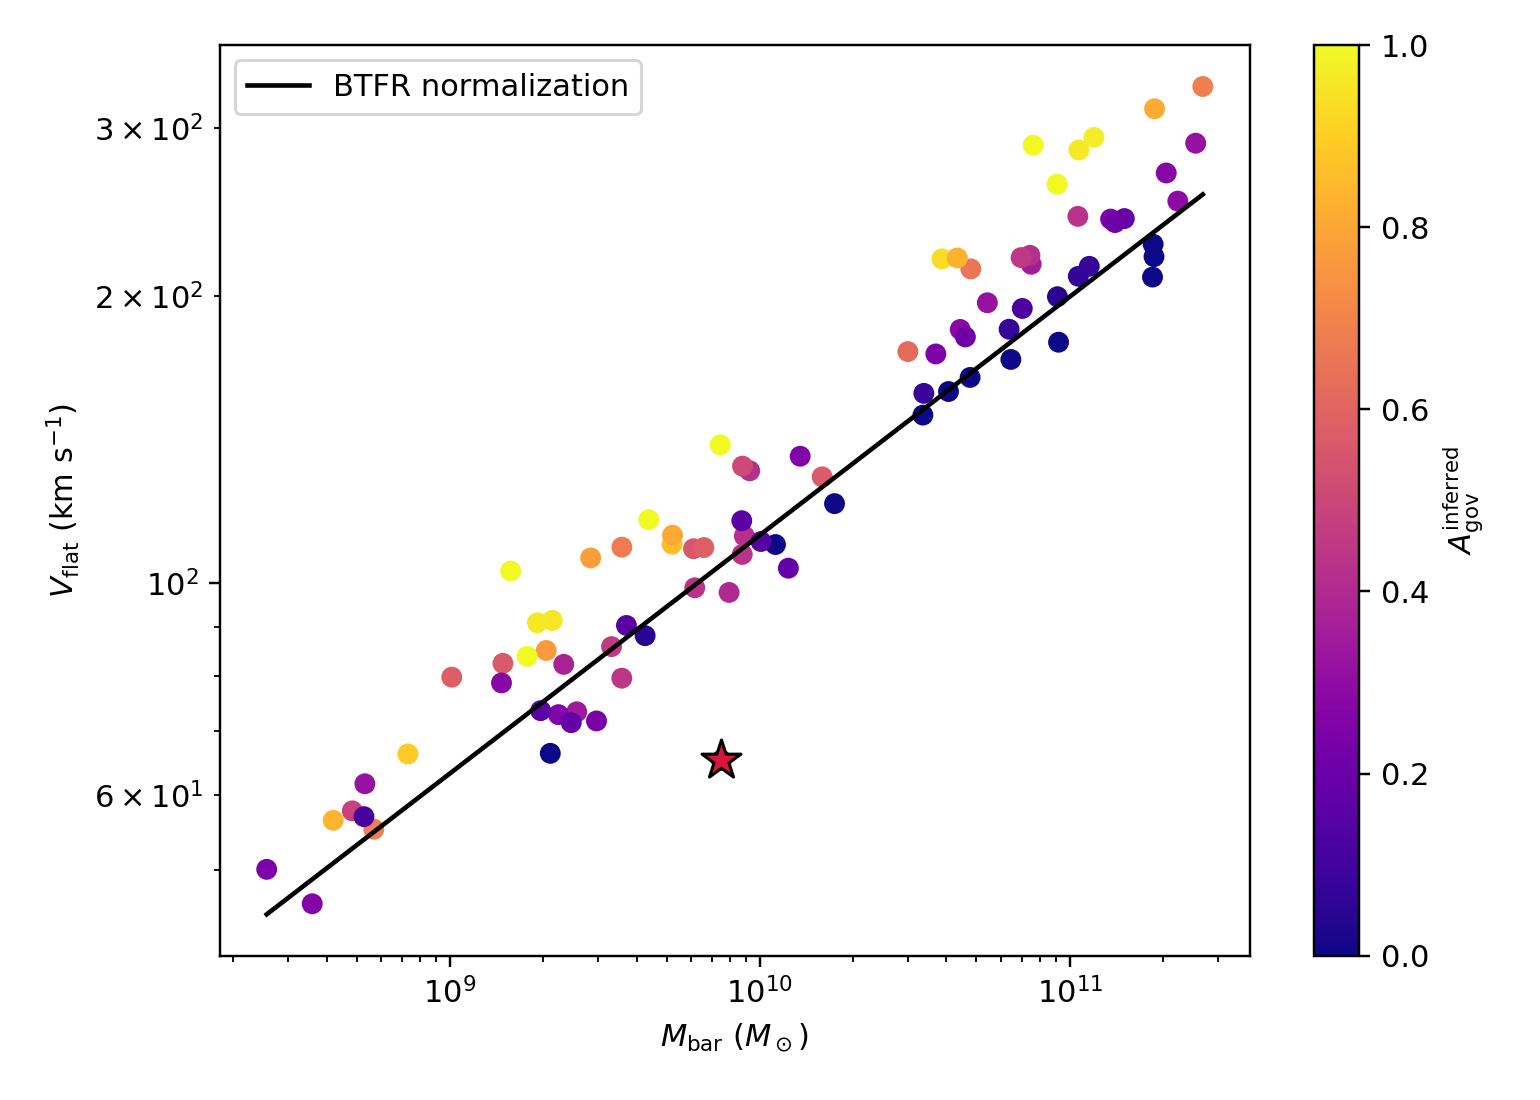
\includegraphics[width=0.92\linewidth]{figures/fig_2_btfr_by_governor_class.png}
\caption{BTFR plane colored by inferred governor activation. The coloring is descriptive because $A_{{\rm inferred}}$ is partly constructed from the same observed velocity on the vertical axis; it is not an independent validation plot.}
\label{fig:btfr-governor}
\end{figure}


\section{Robustness and Limitations}

The threshold grid scans stellar-fraction, surface-density, gas-fraction, and H~I-extent breakpoints with fixed logistic slopes. Each grid point is scored against $A_{\rm inferred}$, not against the descriptive maturity class. The score combines mean-squared prediction error with diagnostic penalties that require low predicted activation for juvenile systems and high predicted activation for a substantial mature subset. These penalties do not replace the fit to $A_{\rm inferred}$; they reject activation surfaces that fit numerically only by allowing physically wrong behavior, such as sending gas-rich juvenile systems through the mature channel.

\begin{table}[H]
\centering
\caption{Selected product-gate maturation model. The MSE and $\rho$ ranges summarize the ten highest-ranked grid points, so the table reports the selected surface without repeating near-identical rows.}
\scriptsize
\resizebox{\textwidth}{!}{%
\begin{tabular}{llccccccc}
\toprule
Rank & Variant & $f_{*,c}$ & $\log\Sigma_{b,c}$ & $f_{\rm gas,c}$ & $(R_{\rm H\,I}/R_d)_c$ & Slopes & MSE range & $\rho$ range \\
\midrule
best & product\_star\_sigma\_gas\_hi & 0.25 & 7.80 & 0.75 & 7.5 & $k_*=10$, $k_\Sigma=4$, $k_{\rm gas}=8$, $k_{\rm H\,I}=1.0$ & 0.183--0.199 & 0.075--0.146 \\
\bottomrule
\end{tabular}%
}
\end{table}

The selected surface has $f_{*,c}=0.25$, $\log\Sigma_{b,c}=7.8$, $f_{\rm gas,c}=0.75$, and $(R_{\rm H\,I}/R_d)_c=7.5$. Its diagnostics are MSE=0.183 and Spearman $\rho=0.146$; this is modest ordering with substantial unexplained scatter, not validation or confirmation. Details of the grid search are in Appendix A.

\paragraph{Clipping audit.} The clipped $A_{\rm inferred}$ distribution contains 12 galaxies clipped to 0, 6 galaxies clipped to 1, and 69 remaining within the interval. Thus 18 of 87 galaxies are boundary-coded rather than continuously inferred from the data. Only 69 of 87 galaxies remain in the open interval, so $A_{\rm inferred}$ is not a reliable continuous regression target in the current normalization. The unclipped activation proxy spans -0.19 to 1.57 with median 0.34; therefore the vertical concentrations at 0 and 1 are partly consequences of the normalization and clipping rule. Sensitivity of the fit to clipping remains a central limitation.

\begin{table}[H]
\centering
\scriptsize
\caption{Baseline comparison for preliminary SPARC activation ordering.}
\resizebox{\textwidth}{!}{%
\begin{tabular}{lrrl}
\toprule
Model & MSE & Spearman $\rho$ & Note \\
\midrule
constant mean baseline & 0.104 & nan & no maturity variables \\
stellar fraction alone & 0.255 & -0.018 & $f_*$ only \\
gas fraction alone & 0.255 & -0.018 & $1-f_{\rm gas}$ only \\
surface density alone & 0.291 & -0.366 & $\log\Sigma_b$ only \\
H~I extent alone & 0.157 & 0.497 & $R_{\rm H\,I}/R_d$ suppressor only \\
reduced two-variable model & 0.248 & -0.018 & $f_*$ and $f_{\rm gas}$ \\
selected product gate & 0.183 & 0.146 & four logistic gates \\
simple linear regression & 0.084 & 0.490 & linear fit to four maturity variables \\
\bottomrule
\end{tabular}%
}
\end{table}

The selected product gate has higher MSE than the constant-mean baseline in Table 3, so MSE should not be read as evidence for a successful continuous regression. Because the endpoint target is heavily clipped, low/high activation classification is the more appropriate first use of the diagnostic. The four-gate form is retained only as a hypothesis-generating ordering device; the marginal improvement over stellar fraction or gas fraction alone must be tested in an independent resolved-observation sample.

\paragraph{Resampling and sensitivity.} A repeated k-fold cross-validation diagnostic using fixed predictions gives held-out prediction error $\mathrm{MSE}=0.183\pm0.048$ across folds. A bootstrap confidence interval for Spearman $\rho$ is approximately -0.094--0.311; threshold stability across resamples is only a preliminary audit because the current grid was selected on the same sample. Inclusion/exclusion sensitivity for the known asymmetric geometry case gives MSE=0.183 with the case included and MSE=0.185 for the case excluded. asymmetric/warped-system exclusions and alternate quality cuts are required before any stronger claim. Full uncertainty propagation remains deferred; distances, inclinations, $v_{\rm flat}$, stellar mass-to-light ratio, gas mass, disk scale length, H~I radius, and evaluation radius must be propagated before galaxies near $A_{\rm inferred}=0$ are interpreted as physically distinct from low positive values.

\section{Corrected Activation-Rank Diagnostic}

The corrected activation-rank calculation is included as a supervised reparameterization diagnostic. It asks whether the same corrected scalar target can be ordered by a latent coordinate after expanding clipped endpoints and adding maturity, reservoir, and angular-momentum context. The baseline product gate has Spearman $\rho=0.146$ against corrected $A_{\rm inferred}$. The selected corrected rank coordinate reaches full-fit rank Spearman $\rho=0.981$ and five-fold out-of-fold rank Spearman $\rho=0.968$; the out-of-fold bounded RMSE is 0.081.

This improvement is manuscript-relevant because it shows that the corrected endpoint target contains an orderable scalar structure. It is not independent validation: the coordinate is trained on corrected $A_{\rm inferred}$, and its success does not promote the governor, does not change the mature velocity law, and does not replace the required same-object H~I morphology and kinematic test. The selected rank coordinate uses angular-momentum context; M59 backbone context is not used by the selected model, so proxy/context rows are not promoted to direct validation. UGC07125 remains excluded from clean scalar interpretation, with $A_{\rm inferred}=0.000$ and bounded corrected-rank value $A_{\rm bounded,M70}=0.000$.


\begin{figure}[t]
\centering
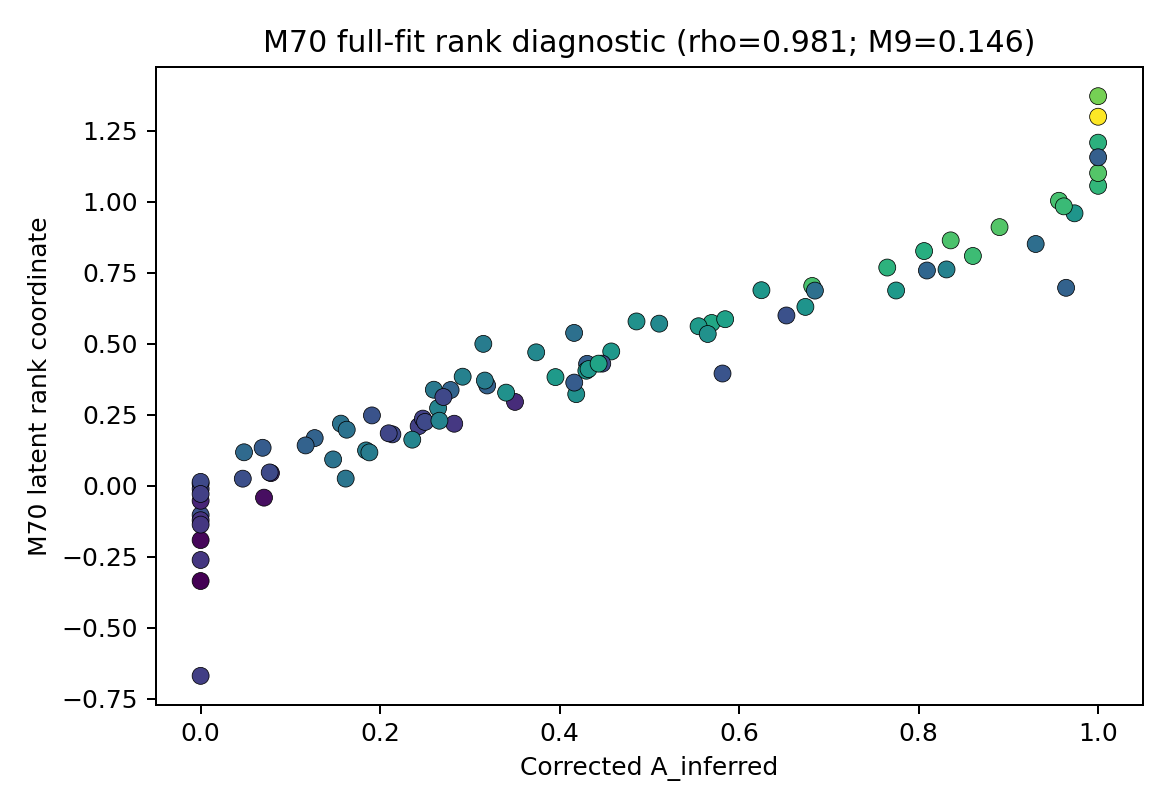
\includegraphics[width=0.92\linewidth]{figures/fig_m70_rank_reparameterization.png}
\caption{Corrected activation-rank reparameterization diagnostic. The panels compare corrected inferred activation with the supervised latent rank coordinate and its bounded version. The figure is a diagnostic of orderability within the current scalar target, not independent validation of the physical governor.}
\label{fig:m70-rank}
\end{figure}



\begin{figure}[t]
\centering
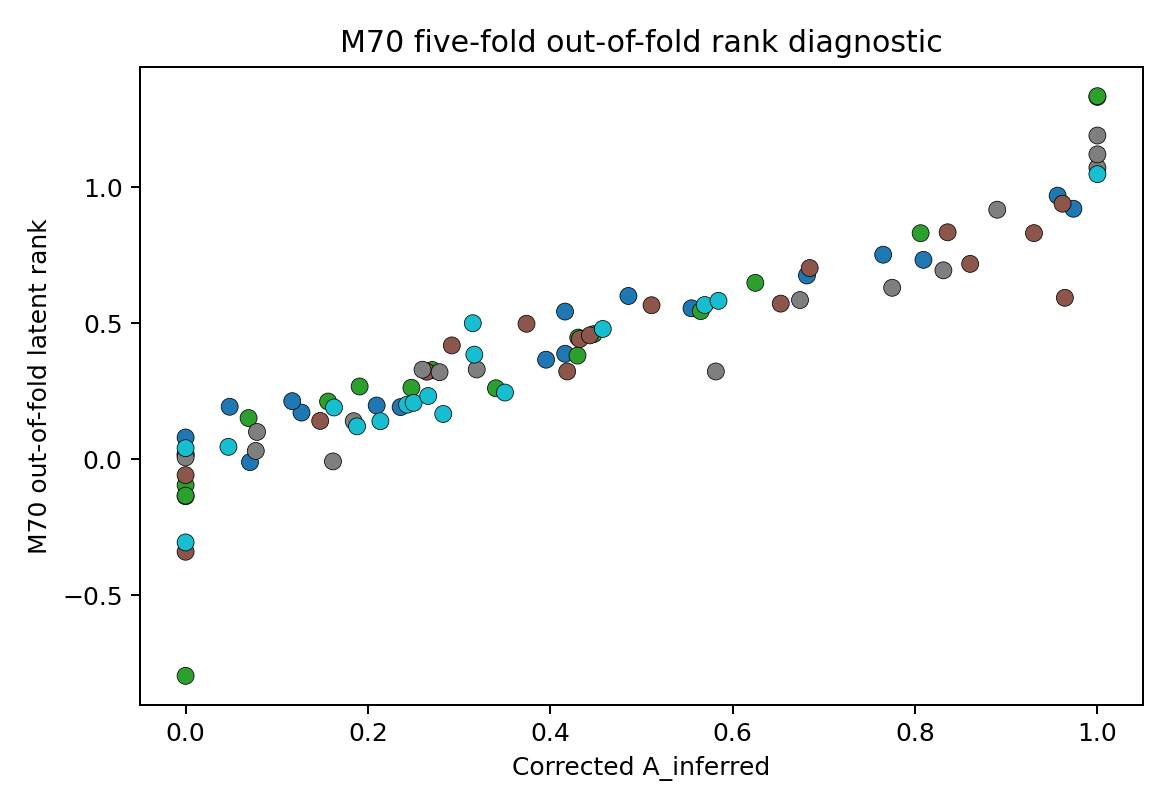
\includegraphics[width=0.92\linewidth]{figures/fig_m70_cv_rank_diagnostic.png}
\caption{Five-fold out-of-fold corrected-rank diagnostic. The out-of-fold comparison guards against a purely in-sample display, but it remains trained on the same corrected activation target and should be read as a reparameterization audit rather than an external validation test.}
\label{fig:m70-cv-rank}
\end{figure}


\section{A Testable Maturation Sequence}

The juvenile-to-mature hypothesis predicts that gas consumption and disk settling raise the activation state. A single-zone toy track captures the direction of the observable sequence: a gas-rich protogalaxy begins with low $f_*$ and low $A_{\rm pred}$, then approaches the mature BTFR as star formation and structural settling increase the activation gate.


\begin{figure}[t]
\centering
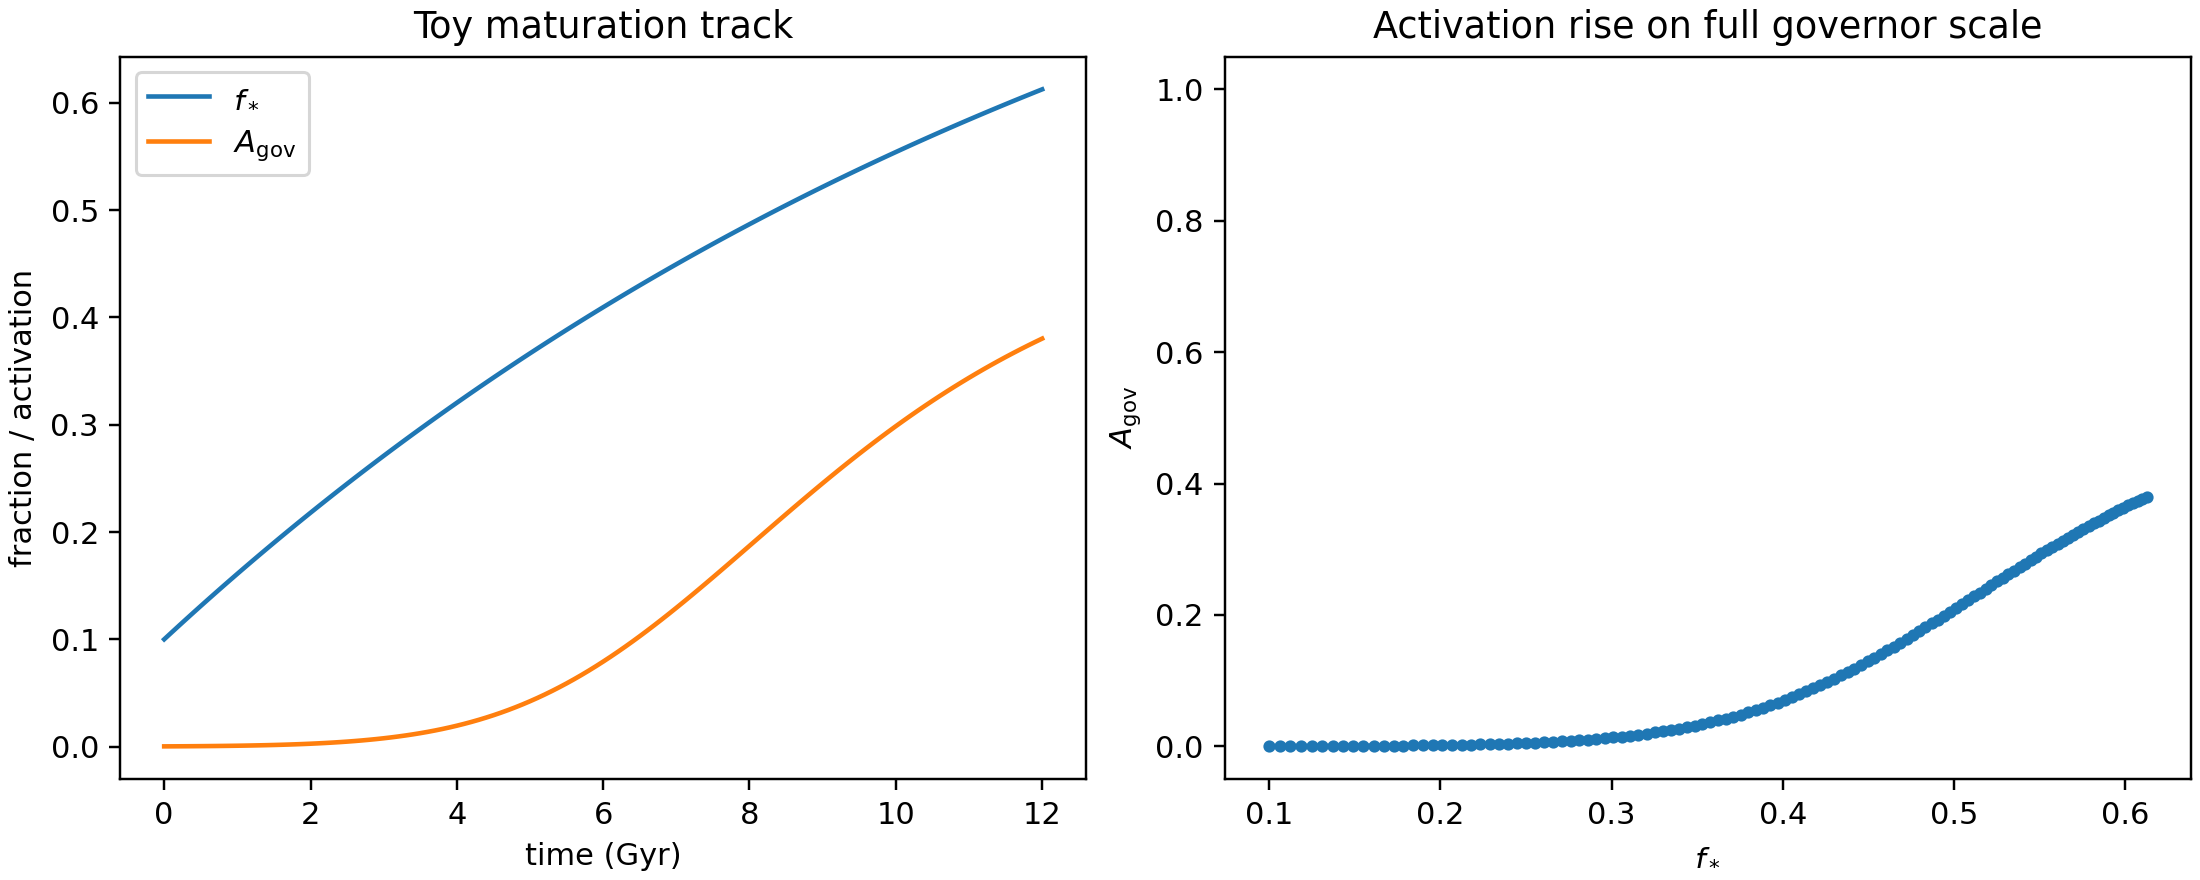
\includegraphics[width=0.92\linewidth]{figures/fig_5_maturation_track_simulation.png}
\caption{Conceptual toy trajectory, not a reconstructed evolutionary history. The track illustrates a hypothesized direction in maturity space. Any assumed evolution of baryonic mass, disk scale length, and surface density is a toy prescription, not a source-derived history.}
\label{fig:maturation-track}
\end{figure}



\begin{figure}[t]
\centering
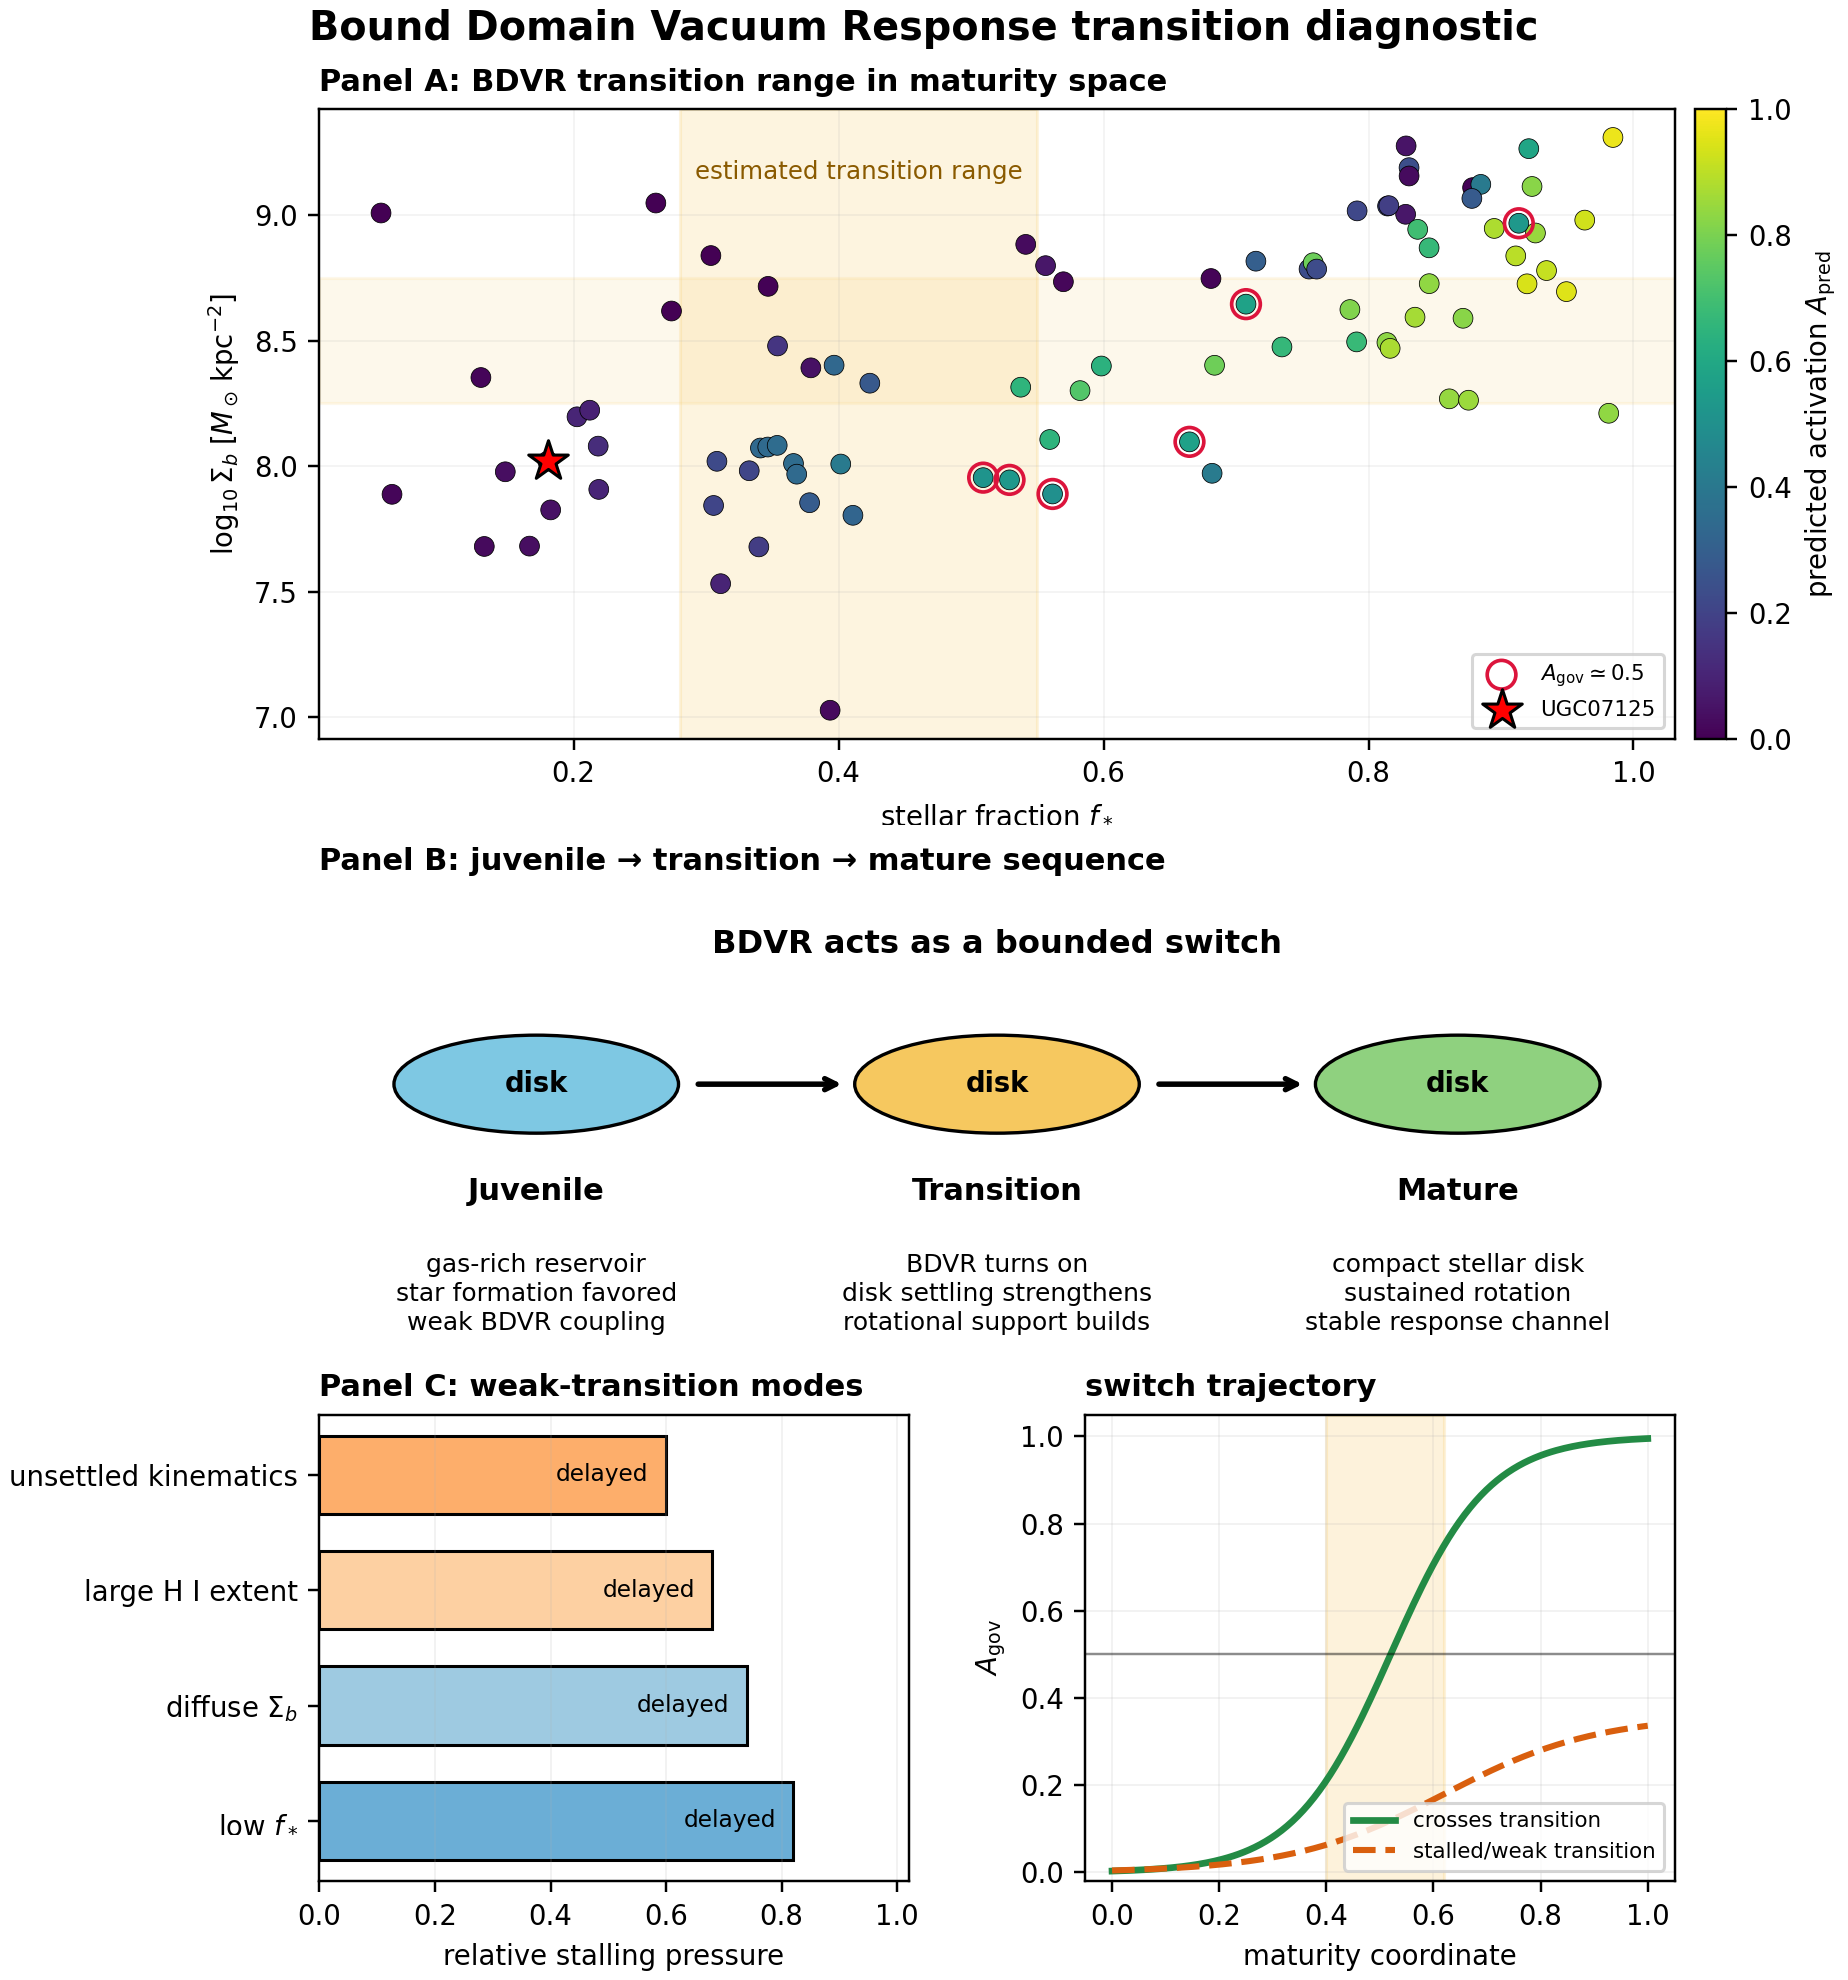
\includegraphics[width=0.92\linewidth]{figures/fig_6_bdvr_transition_multipanel.png}
\caption{Multi-panel BDVR transition diagnostic. Panel A marks the maturity-space transition range where stellar conversion and surface-density buildup begin to open the response channel. Panel B walks through the juvenile, transition, and mature sequence. Panel C shows weak-transition modes that leave gas-rich or diffuse systems below sustained mature rotational support.}
\label{fig:bdvr-transition-multipanel}
\end{figure}


\section{External Proxy Consistency Checks and Target Selection}

External surveys provide proxy consistency checks and candidate-selection channels, not direct validation of BDVR activation. THINGS is the most relevant pilot because it contains resolved H~I maps, but N=8 is exploratory and motivates a larger homogeneous audit. MaNGA supplies stellar and ionized-gas IFU proxies, not outer H~I rotation or direct governor activation. xGASS/xCOLD GASS is used for candidate selection and gas-state ordering. ATLAS3D fast and slow rotators are endpoint controls, not direct disk-galaxy analogs or evidence for a BDVR maturation sequence.

\begin{table}[H]
\centering
\scriptsize
\caption{External survey context for target selection; these rows are not BDVR activation tests.}
\resizebox{\textwidth}{!}{%
\begin{tabular}{p{0.16\textwidth}p{0.28\textwidth}p{0.30\textwidth}p{0.26\textwidth}}
\toprule
Dataset & Context & Qualitative use & Direct-test limitation \\
\midrule
THINGS & Low-$A_{\rm pred}$ galaxies should have higher H~I disturbance. & N=8 resolved-H~I pilot; useful for selecting an asymmetry follow-up sample. & Too small for a statistically meaningful BDVR activation test. \\
MaNGA & Dense, low-sSFR systems occupy an earlier-type/settled locus. & Large IFU proxy sample for target triage and inner-settling context. & MaNGA supplies stellar and ionized-gas IFU proxies, not outer H~I rotation. \\
ATLAS3D & Fast and slow rotators bracket mixed-support and pressure-supported endpoints. & Endpoint controls for language about rotational support channels. & Early-type fast/slow rotators are not disk-galaxy activation tests. \\
xGASS/xCOLD GASS & Gas fraction and depletion track ordinary gas-richness/maturity trends. & Candidate selection and gas-state ordering for future resolved follow-up. & Gas-fraction correlations are partly definitional, not independent BDVR evidence. \\
\bottomrule
\end{tabular}%
}
\end{table}

This table is a target-selection map, not a hypothesis-test table. External surveys show qualitative trends consistent with the idea that gas-rich systems are less dynamically settled, but they do not provide direct tests of the BDVR activation hypothesis. As context, the ladder still separates gas-rich diffuse systems, settling disks, mixed-support fast rotators, and pressure-supported spheroids into qualitatively different response channels. THINGS has only an N=8 pilot overlap, MaNGA uses an invented scalar proxy rather than outer H~I rotation, xGASS/xCOLD GASS gas-fraction correlations are partly definitional, and ATLAS3D fast/slow rotators are endpoint controls rather than disk-galaxy activation tests.

\section{Candidate Targets}

The current direct audit records 2 low-activation candidate(s); DDO161 is retained as the cleaner juvenile-forming contrast. The broader ladder ranks 8 THINGS resolved-H~I proxy rows, 80 xGASS/xCOLD GASS gas-maturity rows, 80 MaNGA scalar/IFU proxy rows, and ATLAS3D control endpoints in a unified 70-row synthesis table. The 70-row synthesis table reports candidate pools and controls after dataset-specific ranking; every candidate still requires geometry or outer-curve verification before direct scalar interpretation.

\begin{table}[H]
\centering
\scriptsize
\caption{Direct SPARC low-activation audit.}
\resizebox{\textwidth}{!}{%
\begin{tabular}{lrrrrrrl}
\toprule
Galaxy & $A_{\rm inferred}$ & $A_{\rm pred}$ & $f_*$ & $f_{\rm gas}$ & $R_{\rm H\,I}/R_d$ & BTFR offset & Status \\
\midrule
DDO161 & 0.000 & 0.013 & 0.130 & 0.870 & 8.76 & -0.060 & clean juvenile-forming contrast; resolved H~I follow-up still required \\
UGC07125 & 0.000 & 0.057 & 0.180 & 0.820 & 6.82 & -0.205 & excluded from clean scalar test: side-dependent H~I/stellar geometry; W side warped, E side not warped \\
\bottomrule
\end{tabular}%
}
\end{table}

\begin{table}[H]
\centering
\scriptsize
\caption{Analog-search channels.}
\resizebox{\textwidth}{!}{%
\begin{tabular}{lllrrl}
\toprule
Channel & Dataset & Role & N searched & Candidate count & Next action \\
\midrule
SPARC direct audit & SPARC & direct & 87 & 2 & resolved H~I and velocity-field check \\
Resolved H~I & THINGS & proxy & 8 & 8 & homogeneous H~I asymmetry audit \\
Gas maturity & xGASS/xCOLD GASS & proxy & 80 & 80 & rotation-curve and H~I follow-up \\
Scalar/IFU screen & MaNGA & proxy & 80 & 80 & gas and outer-curve completion \\
Endpoint control & ATLAS3D & control & 80 & 80 & contrast pressure-supported channel \\
\bottomrule
\end{tabular}%
}
\end{table}

\begin{table}[H]
\centering
\scriptsize
\caption{Top low-activation follow-up candidates and juvenile-forming contrasts.}
\resizebox{\textwidth}{!}{%
\begin{tabular}{llrlll}
\toprule
Candidate & Dataset & Score & Has H~I map & Has IFU & Priority \\
\midrule
DDO161 & SPARC & 0.871 & N & N & Clean juvenile-forming contrast \\
12700-12701 & MaNGA & 0.836 & N & Y & High---follow-up target \\
9091-6103 & MaNGA & 0.829 & N & Y & High---follow-up target \\
GASS102001 & xGASS/xCOLD GASS & 0.827 & N & N & High---follow-up target \\
UGC07125 & SPARC & 0.823 & N & N & Excluded from clean scalar test---side-dependent H~I/stellar geometry \\
8611-6104 & MaNGA & 0.822 & N & Y & High---follow-up target \\
GASS108119 & xGASS/xCOLD GASS & 0.792 & N & N & Medium---proxy screen \\
8139-3703 & MaNGA & 0.785 & N & Y & Medium---proxy screen \\
8617-12705 & MaNGA & 0.781 & N & Y & Medium---proxy screen \\
8619-12704 & MaNGA & 0.778 & N & Y & Medium---proxy screen \\
\bottomrule
\end{tabular}%
}
\end{table}

The tables separate immediate activation checks from follow-up targets and excluded boundary objects. Direct SPARC rows already have activation, baryon, H~I-extent, and BTFR coordinates, but published geometry determines whether those scalar coordinates are clean. External candidates are ranked follow-up targets: gas-selected rows need outer rotation and resolved H~I information, IFU rows need gas and outer-curve completion, and endpoint/control rows test the boundary of the maturation sequence rather than direct disk activation.

\section{Observational Predictions and Falsification Program}

\textbf{Headline falsification test.} The strongest prospective test is resolved H~I asymmetry and settling: low-$A_{\rm pred}$ galaxies selected before observation should show systematically larger H~I asymmetry, stronger approaching/receding mismatch, larger centroid offsets, larger warp or position-angle variation, or higher turbulent/dispersion support than mass-matched high-$A_{\rm pred}$ controls. The current SPARC thresholds are retrospective and are not independent falsification tests until fixed before a new sample is measured.

Predictions already testable with SPARC concern scalar locations in $A_{\rm pred}$, $A_{\rm inferred}$, and BTFR response. Predictions requiring resolved H~I concern asymmetry, warp or position-angle variation, approaching/receding rotation-curve mismatch, and centroid offsets. Predictions requiring IFU plus outer rotation curves concern velocity dispersion and inner settling. High-redshift predictions require different tracers and calibrations and should be treated as prospective tests rather than retrospective thresholds. The decisive new dataset is approximately 20 low-$A_{\rm pred}$ targets and approximately 20 mass-matched high-$A_{\rm pred}$ controls with resolved H~I maps, approaching/receding rotation curves, velocity-dispersion estimates, H~I asymmetry, warp and position-angle variation, stellar/H~I centroid offsets, and consistent distances and inclinations. No existing public table currently combines all of these measurements homogeneously for the required objects.

\begin{enumerate}
\item \textbf{Prediction 1 (mature systems).} Among galaxies with $f_*>0.3$, $\log\Sigma_b>8.0$, $f_{\rm gas}<0.5$, and $R_{\rm H\,I}/R_d<5.0$, less than 5\% should have $A_{\rm inferred}<0.2$.
\item \textbf{Prediction 2 (juvenile systems).} Among galaxies with $f_*<0.2$ and $R_{\rm H\,I}/R_d>6.0$, less than 10\% should have $A_{\rm inferred}>0.6$.
\item \textbf{Prediction 3 (H~I asymmetry).} In a sample of 20 low-$A_{\rm pred}$ galaxies and 20 matched high-$A_{\rm pred}$ controls, the median H~I asymmetry should be at least 0.1 higher in the low-activation sample, with a Mann--Whitney $p<0.05$.
\item \textbf{Prediction 4 (high-redshift gas-rich disks).} In a mass-matched sample at $z>1$, the median $\alpha_{\rm BTFR}<0.8$ for galaxies with $f_{\rm gas}>0.7$.
\end{enumerate}

The governor hypothesis fails if, after controlling for baryonic mass and measurement quality, low predicted activation is not associated with reduced rotational response or with independently measured dynamical immaturity. It also fails if dynamically settled, compact, stellar-rich disks frequently occupy the low-response channel. Thresholds above are retrospective when selected from the current SPARC sample and prospective only when fixed before a new resolved-observation campaign.

\section{Discussion: Relation to MOND, the RAR, and Disk Evolution}

The acceleration scale and BTFR-like term have established precedent in Milgromian dynamics and RAR work. This paper does not claim that BDVR independently rediscovers ordinary scaling relations. The RAR gas-richness trend already shows that gas-rich systems occupy a recognizable sequence in acceleration space; the proposed difference is the threshold-and-settling interpretation, namely that resolved disk organization should determine which gas-rich, extended systems remain in a low-response channel. The current scalar evidence is too weak to distinguish that interpretation from a standard gas-richness trend. A reader could reasonably ask why not use stellar fraction or gas fraction alone: Table 3 shows that those one-variable proxies have similar rank information, and the four-gate model offers only marginal improvement. The product gate is therefore a target-selection hypothesis, not a demonstrated new scaling law. In ordinary $\Lambda$CDM hydrodynamic simulations, disk settling also correlates with gas fraction, surface density, and velocity dispersion; Toomre-style stability language is useful only as motivation for future resolved disk-settling variables, not as the definition of $Q_{\rm eff}$ here. The distinguishing observation is whether same-object resolved H~I asymmetry, velocity-field mismatch, and settling measurements predict the normalized support residual after controlling for standard mass, size, and measurement-quality variables.

\section{Conclusions}

\begin{sloppypar}
The present analysis motivates, but does not establish, the hypothesis that any additional BDVR-like rotational response is not universal across baryonic disks. The scalar SPARC diagnostics provide only modest evidence for an ordering in which gas-rich and H~I-extended systems occupy a lower predicted-response channel; the severe clipping limitation in Section 7 makes this a low/high activation screen, not a continuous physical activation measurement. The decisive test requires resolved same-object H~I morphology and kinematics that are not presently available in a sufficiently complete homogeneous sample. The next paper-worthy result is therefore observational: approximately 20 low-$A_{\rm pred}$ targets, approximately 20 mass-matched high-$A_{\rm pred}$ controls, resolved H~I maps, side-specific rotation curves, dispersion estimates, asymmetry measures, warp/position-angle variation, centroid offsets, and consistent distances and inclinations. If that dataset does not link low predicted activation to reduced response or independently measured dynamical immaturity, the governor hypothesis fails.
\end{sloppypar}

\clearpage
\appendix

\section{Threshold grid-search details}

The grid search is a diagnostic selection layer, not a fundamental equation. It scans a compact set of stellar-fraction, surface-density, gas-fraction, and H~I-extent breakpoints with fixed logistic slopes, scores each surface against $A_{\rm inferred}$, and applies diagnostic penalties only to exclude numerically adequate surfaces with physically wrong channel behavior. The selected product gate is then carried into candidate selection and external proxy consistency checks.

\section{Test Results Summary}

The SPARC quality-1 governor run contains 87 galaxies. The toy maturation diagnostic classifies 14 dynamically immature systems, 32 transition systems, and 41 mature systems. The selected threshold surface has mean squared error 0.183 and Spearman $\rho=0.146$. The external proxy synthesis contributes 11275 usable proxy measurements across five survey stages, with the external sequence ordered by gas fraction, surface density, angular-momentum support, and pressure support.

\section{Dataset Descriptions}

SPARC supplies the quality-1 disk-galaxy flat velocities and baryonic variables used for direct governor activation inference. THINGS supplies resolved H~I structure maps for pilot disturbance and side-to-side kinematic diagnostics. MaNGA supplies a large IFU scalar sample used for surface-density and star-formation proxy activation. ATLAS3D supplies early-type angular-momentum measurements used for fast-rotator bridge and pressure-channel diagnostics. xGASS and xCOLD GASS supply atomic and molecular gas measurements used for gas-depletion maturity ordering.

\section{Machine-Readable Artifacts}

\begin{sloppypar}
The manuscript package includes machine-readable source tables copied beside the manuscript for reproducibility:
\begin{itemize}
\item \texttt{m9\_summary.json}
\item \texttt{m9\_inferred\_activation.csv}
\item \texttt{m9\_governor\_threshold\_fits.csv}
\item \texttt{m9\_governor\_predictions.csv}
\item \texttt{m9\_gate\_diagnostics.csv}
\item \texttt{m9\_ugc07125\_governor\_audit.csv}
\item \texttt{m9\_falsification\_candidates.csv}
\item \texttt{m16\_external\_validation\_summary\_table.csv}
\item \texttt{m16\_external\_validation\_claim\_boundaries.csv}
\item \texttt{m16\_external\_validation\_synthesis.json}
\item \texttt{m17\_ugc07125\_prototype\_vector.json}
\item \texttt{m17\_sparc\_direct\_analog\_audit.csv}
\item \texttt{m17\_ugc07125\_analog\_synthesis.csv}
\item \texttt{m17\_ugc07125\_analog\_synthesis.json}
\item \texttt{m70\_summary.json}
\item \texttt{m70\_predictions.csv}
\item \texttt{m70\_cv\_predictions.csv}
\item \texttt{m70\_reparameterization\_fits.csv}
\item \texttt{m70\_fold\_metrics.csv}
\item \texttt{m70\_equation\_specification.md}
\end{itemize}
\end{sloppypar}

\begin{thebibliography}{99}
\bibitem{toomre1964} Toomre, A. 1964, On the gravitational stability of a disk of stars, Astrophysical Journal, 139, 1217.
\bibitem{kennicutt1998} Kennicutt, R. C. 1998, The global Schmidt law in star-forming galaxies, Astrophysical Journal, 498, 541.
\bibitem{romeo2017} Romeo, A. B., and Mogotsi, K. M. 2017, Star-gas stability in nearby spirals, Monthly Notices of the Royal Astronomical Society, 469, 286.
\bibitem{begeman1991} Begeman, K. G., Broeils, A. H., and Sanders, R. H. 1991, Extended rotation curves of spiral galaxies, Monthly Notices of the Royal Astronomical Society, 249, 523.
\bibitem{mcgaugh2005} McGaugh, S. S. 2005, The baryonic Tully-Fisher relation of galaxies with extended rotation curves, Astrophysical Journal, 632, 859.
\bibitem{milgrom1983} Milgrom, M. 1983, A modification of the Newtonian dynamics as a possible alternative to the hidden mass hypothesis, Astrophysical Journal, 270, 365.
\bibitem{famaey2012} Famaey, B., and McGaugh, S. S. 2012, Modified Newtonian Dynamics: successes and challenges, Living Reviews in Relativity, 15, 10.
\bibitem{mcgaugh2016rar} McGaugh, S. S., Lelli, F., and Schombert, J. M. 2016, Radial acceleration relation in rotationally supported galaxies, Physical Review Letters, 117, 201101.
\bibitem{lelli2017rar} Lelli, F., McGaugh, S. S., Schombert, J. M., and Pawlowski, M. S. 2017, One law to rule them all: the radial acceleration relation of galaxies, Astrophysical Journal, 836, 152.
\bibitem{sales2017} Sales, L. V., Navarro, J. F., et al. 2017, The low-redshift galaxy population in the Lambda-CDM hydrodynamical simulation context, Monthly Notices of the Royal Astronomical Society, 464, 2419.
\bibitem{jog1997} Jog, C. J. 1997, Lopsidedness of galactic disks, Astrophysical Journal, 488, 642.
\bibitem{navarro1996} Navarro, J. F., Frenk, C. S., and White, S. D. M. 1996, The structure of cold collisionless halos, Astrophysical Journal, 462, 563.
\bibitem{lelli2016sparc} Lelli, F., McGaugh, S. S., and Schombert, J. M. 2016, SPARC: Mass Models for 175 Disk Galaxies, Astronomical Journal, 152, 157.
\bibitem{walter2008things} Walter, F. et al. 2008, THINGS: The H~I Nearby Galaxy Survey, Astronomical Journal, 136, 2563.
\bibitem{bundy2015manga} Bundy, K. et al. 2015, Overview of the SDSS-IV MaNGA Survey, Astrophysical Journal, 798, 7.
\bibitem{cappellari2011atlas3d} Cappellari, M. et al. 2011, The ATLAS3D Project, Monthly Notices of the Royal Astronomical Society, 413, 813.
\bibitem{catinella2018xgass} Catinella, B. et al. 2018, xGASS: total cold gas scaling relations, Monthly Notices of the Royal Astronomical Society, 476, 875.
\bibitem{saintonge2017xcold} Saintonge, A. et al. 2017, xCOLD GASS: molecular gas scaling relations, Astrophysical Journal Supplement, 233, 22.
\end{thebibliography}

\end{document}
